\chapter{Case Study}
This chapter contains the focus of this report.

\section{High-Level Synthesis}
High-Level Synthesis is a way to design hardware using high abstraction layers. Traditionally for FPGA hardware, you work in structural, RTL and behavioural layers which are all very close to the hardware. A high amount of detail is needed when designing in these layers. A higher abstraction layer provides a way to design and create systems without going into too much  into the detailed layers. The higher abstraction layer is made possible by the High-Level synthesis, that is translating high level design into RTL level design. The high level layer is typically designed in C++, C or system C. A figure from The Zynq Book\cite{crockett2014the} explains this well and can be seen in figure \ref{fig:abslevels}.
\begin{figure}[H]
\centering
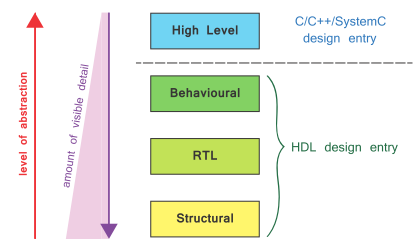
\includegraphics[scale=1]{billeder/abslevels}
\caption{Abstraction levels in FPGA designs from The Zynq Book}
\label{fig:abslevels}
\end{figure}
An interesting question is then: "Why use High-Level synthesis for hardware when the environment is C++, C etc. ?". The short answer to that question would be that hardware gives you tight control with two fundamental metrics in your design: Area (or resource cost) and Speed. The goal is to have the highest speed (or throughput) with the lowest possible area requirement, that still satisfies your design solution.\\
Using a tool like Vivado HLS, it is possible to analyse and compare design against each other. The tool also offers a wide range of optimisation possibilities. The  optimisation possibilities are also known as optimisation directives. These directives can be found in table 1-23 in the Vivado Design Suite User Guide\footnote{http://www.xilinx.com/products/design-tools/vivado/integration/esl-design.html}. An small excerpt of these can be found in table \ref{tab:directives}.
\begin{table}[H]
\centering
    \begin{tabular}{|l|p{10cm}|}
    \hline
    Directive  & Description                                                                                                                                                                       \\ \hline
    ALLOCATION & Specify a limit for the number of operations, cores or function used. This can force the sharing of hardware resources and may increase latency                                   \\ \hline
    INLINE     & Inlines a function, removing all function hierarchy. Used to enable logic optimisation across function boundaries and improve latency/interval by reducing function call overhead \\ \hline
    PIPELINE   & Reduces the initiation interval by allowing the concurrent execution of operations within a loop or function                                                                      \\ \hline
    DATAFLOW   & Enables task level pipelining, allowing functions and loops to execute concurrently. Used to minimize interval.                                                                                                                                                                                 \\ \hline
    \end{tabular}
    \caption{Excerpt of table 1-23 from Vivado Design Suite User Guide}
    \label{tab:directives}
\end{table}
The directives have direct influence on some of the design goals with regards to:
\begin{itemize}
\item Area (or Resources)
\item Speed (or Throughput)
\item Maximum clock frequency
\item Latency
\end{itemize}
These metrics will be the basis of the analysis in this project.\\

With the knowledge of the directives, the new question becomes: "How are they implemented into the design?". Directives can either be inserted into the source file as a pragma as can be seen in Listing \ref{lstpragma} or they can be added to the directive file using the tool.
\begin{lstlisting}[caption={Inserting directive into source code.},label=lstpragma]
IRow: for (  int i = 0; i < 3, i++ )
{
	#pragma HLS PIPELINE
	ICol: for ( int j = 0; j < 3, j++)
	{
		...
	}
}
\end{lstlisting}
As an example, pipelining a function like above causes the software to unroll all loops in the hierarchy. It reduces latency as the cost of increasing area. This can be seen in the synthesis report when the software tool has finished the C synthesis.

\section{Example Problem}
\label{sec:example}
The problem chosen in this project is a least squares problem known from the world of optimisation. Least squares are used for regression by finding an estimate $\hat{x}$ that fulfils the equation $A\textbf{x} = \textbf{b}$. This is done using the following equation:
\begin{equation}
\label{leastsquares}
\hat{x} = (A^T * A)^{-1}*A^T*\textbf{b}
\end{equation}
The example is defined as:\\
A = $3 \times 3$~matrix
\[ \left( \begin{array}{ccc}
1 & 2 & 3 \\
3 & 4 & 5 \\
5 & 6 & 8 \end{array} \right)\] \\
b = $3 \times 1$~vector
\[ \left( \begin{array}{c}
4 \\
2 \\
1 \end{array} \right)\]
Solving the problem yields:\\
$\hat{x}$ = $3 \times 1$~vector
\[ \left( \begin{array}{c}
-5 \\
3 \\
1 \end{array} \right)\]
The result contains a negative number. This means the implementation must be done using signed data type. Calculating the inverse matrix in matlab yields:\\
$(A' * A)^{-1}$ = $3 \times 3$~matrix
\[ \left( \begin{array}{ccc}
3 & -5 & 2 \\
-5 & 16.5 & -9.5 \\
2 & -9.5 & 6 \end{array} \right)\] \\
This means the float data type must be used. The float data type is 32 bit and four times as large as the signed char data type originally though to fulfil the requirement. This will increase the resource requirement of the project.

\section{HLS Implementation}
The implementation of a least squares function in HLS is done using the matrix multiplication example found in Lab 1 from the "High-Level Synthesis Flow on Zynq using Vivado" workshop\footnote{http://www.xilinx.com/support/university/vivado/vivado-workshops/Vivado-high-level-synthesis-flow-zynq.html}. The example is modified to fit the project at hand. A function for transposing a matrix is added to the solution along with a function for inverting a matrix. The inverse function is heavily inspired by a solution written by Mr. Ree at stackoverflow.com\footnote{http://stackoverflow.com/questions/983999/simple-3x3-matrix-inverse-code-c}.
The least squares function is defined as:
\begin{lstlisting}[caption={Least Squares function definition},label=lstsquares]
#define MAT_A_ROWS 3
#define MAT_A_COLS 3
#define MAT_B_ROWS 3
#define MAT_B_COLS 1

typedef float mat_a_t;
typedef float result_t;

void leastSquares(mat_a_t a[MAT_A_ROWS][MAT_A_COLS],
      mat_a_t b[MAT_B_ROWS][MAT_B_COLS],
      result_t xhat[MAT_A_ROWS][MAT_B_COLS]);
\end{lstlisting}
with "a" being the A matrix mentioned in section \ref{sec:example}, "b" being the vector and "xhat" being $\hat{x}$. The flow through the function can be described as can be seen in figure \ref{fig:LSFunc}.
\begin{figure}[H]
\centering
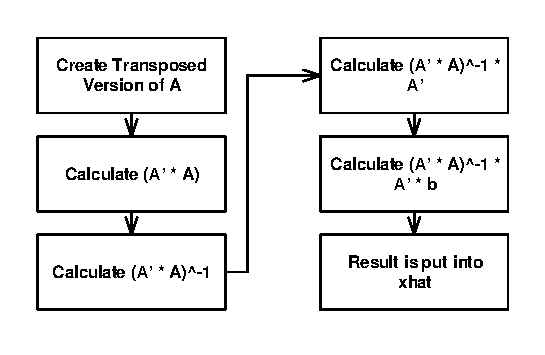
\includegraphics[scale=1]{billeder/leastSquaresFunc}
\caption{Steps in the function calculating least squares}
\label{fig:LSFunc}
\end{figure}
The testbench used in the example project has been modified in order to test the leastSquares function. An excerpt of the testbench is defined as:
\begin{lstlisting}[caption={Excerpt of the testbench code},label=tstbnch]
   mat_a_t in_mat_a[3][3] = {
      {1, 2, 3},
      {3, 4, 5},
      {5, 6 ,8}
   };
   mat_a_t b[3][1] = {
		   {4},
		   {2},
		   {1}
   };
   result_t hw_result[3][1];

#ifdef HW_COSIM
   // Run the AutoESL matrix multiply block
   leastSquares(in_mat_a, b, hw_result);
#endif
\end{lstlisting}
With HW\_COSIM defined, this yields the following output from the leastSquares\_csim.log file:
\begin{verbatim}
   Compiling ../../../../matrixmul_test.cpp in debug mode
   Compiling ../../../../matrixmul.cpp in debug mode
   Generating csim.exe
{
{-5}
{3}
{1}
}
@I [SIM-1] CSim done with 0 errors.
\end{verbatim}
which correspond to the solution found in section \ref{sec:example}. The synthesis report contains the performance as seen in figure \ref{fig:OrigPer} and the resource requirement as seen in figure \ref{fig:OrigUtil}.
\begin{figure}[H]
\centering
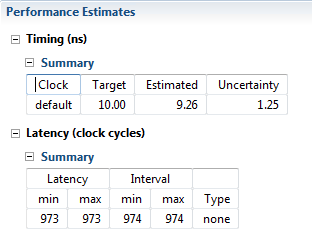
\includegraphics[scale=1]{billeder/OriginalPerform}
\caption{Original Performance with no Optimisation}
\label{fig:OrigPer}
\end{figure}
\begin{figure}[H]
\centering
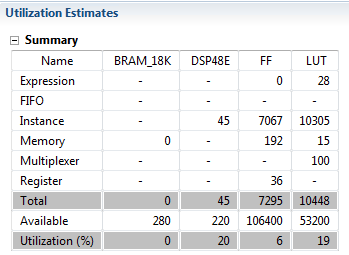
\includegraphics[scale=1]{billeder/OriginalUtil}
\caption{Original Utilization (Resource requirement) with no Optimisation}
\label{fig:OrigUtil}
\end{figure}
In figure \ref{fig:OrigPer} the clock is  estimated to 9.26 ns. This is equivalent to a maximum clock frequency approximately 108 MHz. When doing the final synthesis to RTL the design is further optimised by the tool. This means the maximum clock frequency is approximately 110 MHz with this design. The resource requirement is also reduced along with the latency. This can be seen in figure \ref{fig:OriginalFinal}.
\begin{figure}[H]
\centering
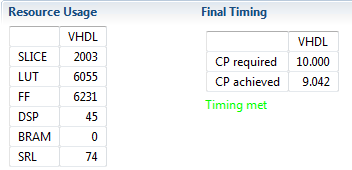
\includegraphics[scale=1]{billeder/OriginalFinal}
\caption{Final synthesis to RTL results}
\label{fig:OriginalFinal}
\end{figure}
Going back to the simulation and using the analysis view and breaking down the report shows which part of the algorithm requires the most resources and which part that gives the most latency. This can be seen in figure \ref{fig:OrigBreak}.
\begin{figure}[H]
\centering
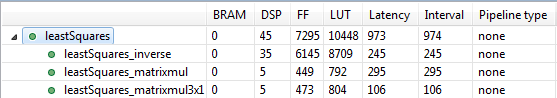
\includegraphics[scale=1]{billeder/OriginalAreaLatency}
\caption{Original breakdown of resources and latency}
\label{fig:OrigBreak}
\end{figure}
With the HLS Implementation complete the task is now to analyse the synthesis and how it can be optimised with regards to resources and latency.
\section{Optimisation}
\subsection{Optimising for speed}
Optimising for speed means analysing figure \ref{fig:OrigBreak} for the functions with the most latency and then evaluate which directive can improve the latency. Evaluating the code with pipelining and dataflow provides insight into the possibilities. The dataflow directive cannot be implemented in the functions. The reason being that the same memory area is read in multiple subsequent instances. The synthesis simply fails in the Vivado HLS tool.
A lot of the calculations are made in for loops. Pipelining these loops will result in fewer cycles overall as explained very well in the Vivado High-Level Synthesis User guide using figure \ref{fig:looppipelining}.
\begin{figure}[H]
\centering
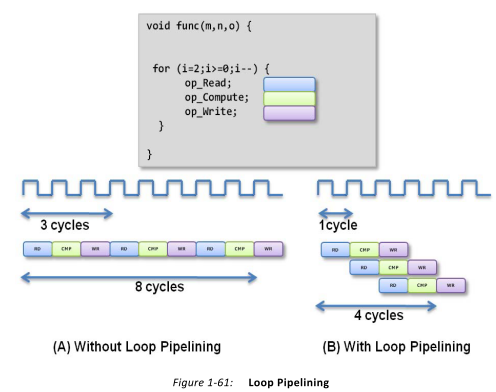
\includegraphics[scale=1]{billeder/looppipelining}
\caption{Loop pipelining from the User Guide}
\label{fig:looppipelining}
\end{figure}
Applying this to the least square function is done by applying the directives to the sub functions used. This can be seen in Listing \ref{pipedirectives}.
\begin{lstlisting}[caption={pipelining directives applied to the least squares sub functions},label=pipedirectives]
set_directive_pipeline "transpose"
set_directive_pipeline "matrixmul"
set_directive_pipeline "matrixmul3x1"
set_directive_pipeline "inverse"
\end{lstlisting}
The synthesis generates a report and inspecting it in analysis mode yields the information seen in figure \ref{fig:SpeedBreak}.
\begin{figure}[H]
\centering
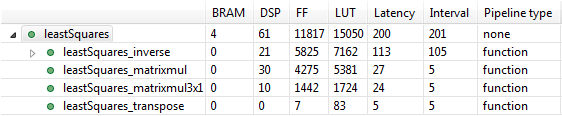
\includegraphics[scale=1]{billeder/SpeedAreaLatency}
\caption{Optimised for speed breakdown of resources and latency}
\label{fig:SpeedBreak}
\end{figure}
It is seen from inspecting the figure that the latency has been improved a lot at the expense of the resources requirements. For number comparison see section \ref{sec:Comp}.
\subsection{Optimising for area}
Optimising for area means repeating the steps from the speed optimisation but evaluating resource requirement instead. It is apparent that the \texttt{leastSquares\_inverse} function is responsible for the largest resource requirement. When evaluating possible solutions, the two directives, inline and allocation can be used. When synthesising the solution it is seen that the tool automatically inlines functions. This can be seen in figure \ref{fig:areainline}.
\begin{figure}[H]
\centering
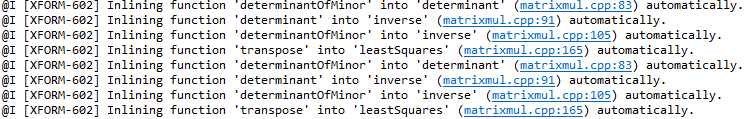
\includegraphics[width  = 1\textwidth]{billeder/inlining}
\caption{Automatic inlining done by the synthesis}
\label{fig:areainline}
\end{figure}
Allocation means constricting the top function to only use the specified amount of instances of a sub function. The allocation is defined as:
\begin{lstlisting}[caption={Allocation directive applied to the least squares inverse sub function },label=allocationdir]
set_directive_allocation -limit 1 
-type function "inverse" determinantOfMinor
\end{lstlisting}
The synthesis generates a report and inspecting it in analysis mode yields the information seen in figure \ref{fig:AreaBreak}.
\begin{figure}[H]
\centering
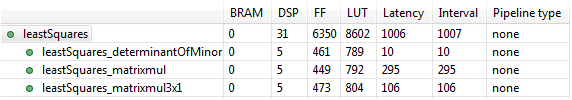
\includegraphics[scale=1]{billeder/AreaAreaLatency}
\caption{Optimised for area breakdown of resources and latency}
\label{fig:AreaBreak}
\end{figure}
It is seen that is is possible to reduce the resource requirement at the expense of latency in figure \ref{fig:AreaBreak}. 
\section{Comparison}
\label{sec:Comp}
The Vivado HLS tool offers a neat way to compare the synthesis reports generated by the different solutions. The comparison can be seen in figure \ref{fig:CompareReports}.
\begin{figure}[H]
\centering
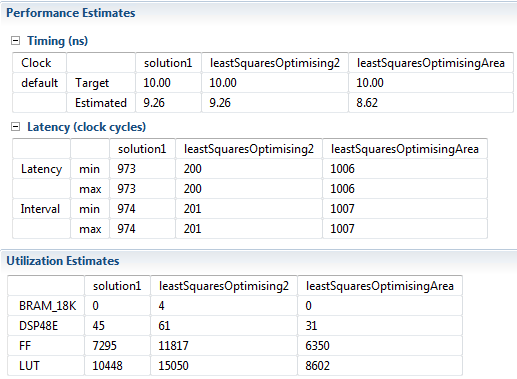
\includegraphics[scale=1]{billeder/CompareReports}
\caption{Comparison between the reports. solution1 is the original unoptimised solution. leastSquaresOptimising2 is the solution optimised for speed. leastSquaresOptimisingArea is the solution optimised for resource requirement.}
\label{fig:CompareReports}
\end{figure}
The comparison gives a good view of how the design metrics can be tuned. Using the different directives it is possible to tune the latency towards the requirement in a specific project. The findings can be written as in table \ref{tab:effects}.
\begin{table}[H]
\centering
    \begin{tabular}{|l|l|l|}
    \hline
    Directive  & Latency    & Area       \\  \hline
    ALLOCATION & $\uparrow$    & $\downarrow$  \\
    INLINE     & $\uparrow$    & $\downarrow$  \\
    PIPELINE   & $\downarrow\downarrow$  & $\uparrow\uparrow$    \\
    DATAFLOW   & Not tested & Not tested \\ \hline
    \end{tabular}
    \caption{Effects of the chosen directives on Latency and Area (Resource Requirement).}
    \label{tab:effects}
\end{table}
The Vivado HLS tool will also do iterative optimisation when generating the RTL code for use in system level projects as seen in figure \ref{fig:OriginalFinal}. This will reduce area further while seeking to maintain the specified latency.